\section{Splitter}
Splitter helps in splitting a Network Service (NS) into multiple sub Network services which can be deployed and instantiated individually on Internet Service Providers (ISPs) located over a vast geographical region spanning multiple domains and are orchestrated by different MANO frameworks. Splitter calls Service Descriptor Transltor if there is a need to translate the NS if it is to be deployed on a different MANO framework. In this work package, a Service Descriptor Splitter (SDS) is implemented which splits the NSD of a network service. SDS takes NSD as an input that contains all the information elements which can be extracted to generate separate NSDs. In the proposed approach, the service graph is extracted from the input NSD and is split into subgraphs that result in a separate NSD which includes a set of elements such as VNFs, Virtual Links (VLs), forwarding graphs of VNFs etc, according to the specific MANO framework.

\subsection{Architecture and Work flow}

Figure \ref{fig:osmschemaclassdiagram}, \ref{fig:osmsplitterclassdiagram}, \ref{fig:pishahangschemaclassdiagram} and \ref{fig:pishahangsplitterclassdiagram} represents class diagrams of OSM and Pishahang. Python base classes are used for different sections of a NSD which encapsulate all the attributes and its values into a single unit which makes it very easy to process. Once the objects are set they are passed to different splitting functions based on there type. We have two different processing units for OSM and SONATA. Figure \ref{fig:splittersequencediagram} shows the sequence diagram of Pishahang splitter. Following are some functions responsible for splitting the NSD.

\begin{itemize}
	\item \textbf{Validate: }Validation of the incoming request from MANO for splitting happens is done before actual splitting. Validation checks if the request has correct VNF ids. It also checks if the list of VNFs specified in the request is matching with the list of VNFs in the original NSD file.
	\item \textbf{Set connection point reference for virtual functions:}After validation, as per the incoming request multiple set of empty NSD objects are created. This step updates the empty NSD objects with connection points. These connection points are either of type “external” or “management”. Each sub NSD will have its own connection points just like its parent NSD.
	\item \textbf{Split Network Functions: }After creating connection points for each sub NSDs, VNF objects are set in the updated NSD objects as per the request from MANO. Each set of VNFs from the request is set in each of the NSD objects. 
	\item \textbf{Split Virtual Links: }When a NSD is splitted into different parts, its topology changes. Change in topology results in changing of Virtual Links. For example if A, B and C are three Nfs and we are splitting them in such a way so that A and B remain in one NSD and C in separate NSD. A virtual link between B and C now does not make sense. So this link should be broken down and B’s output should be connected to the external end point which was connected to C’s input earlier. This function splits these kind of Virtual Links.
	\item \textbf{Split Forwarding Graph: }Once the topology changes, the respective Forwarding graph also changes. Split forwarding graph pulls out the set of connection points and newly created virtual links and sets them in the sub NSDs. The current implementation can split a NSD with three or less VNFs. To maintain the topology of the original NSD, Splitter needs to extract virtual links from the main NSD and create new virtual links for sub NSDs in such a way that the topology of the main NSD is maintained. 
	\item \textbf{Create Sub-NSDs: } The last step is to return the sub-nsds created out of NSD objects.
\end{itemize} 

\begin{figure}
	\centering
	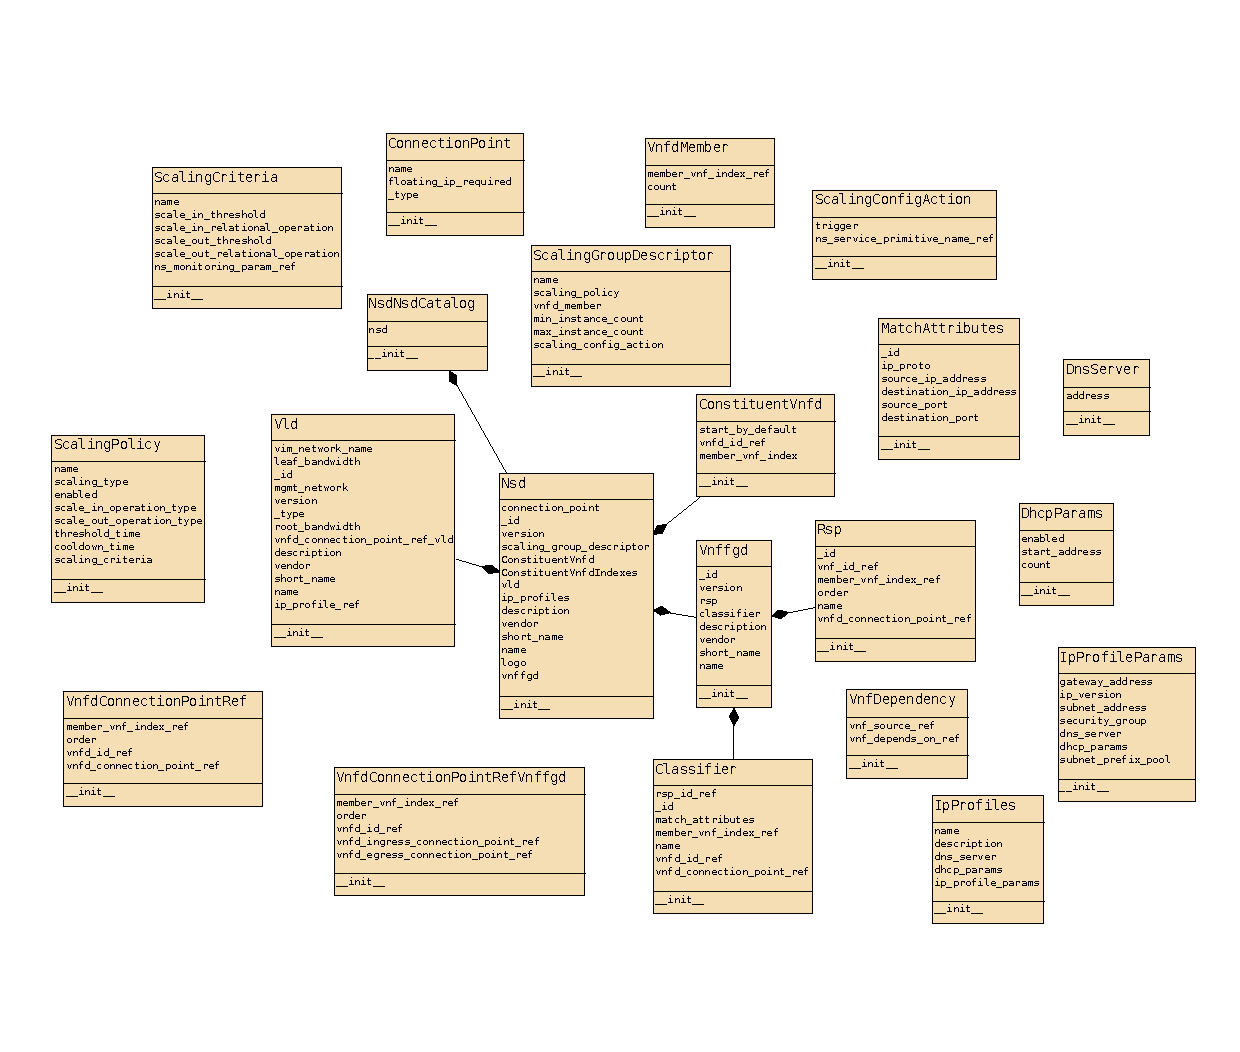
\includegraphics[width=1\linewidth]{../figures/osm-schema}
	\caption{OSM Schema Class Diagram}
	\label{fig:osmschemaclassdiagram}
\end{figure}

\begin{figure}
	\centering
	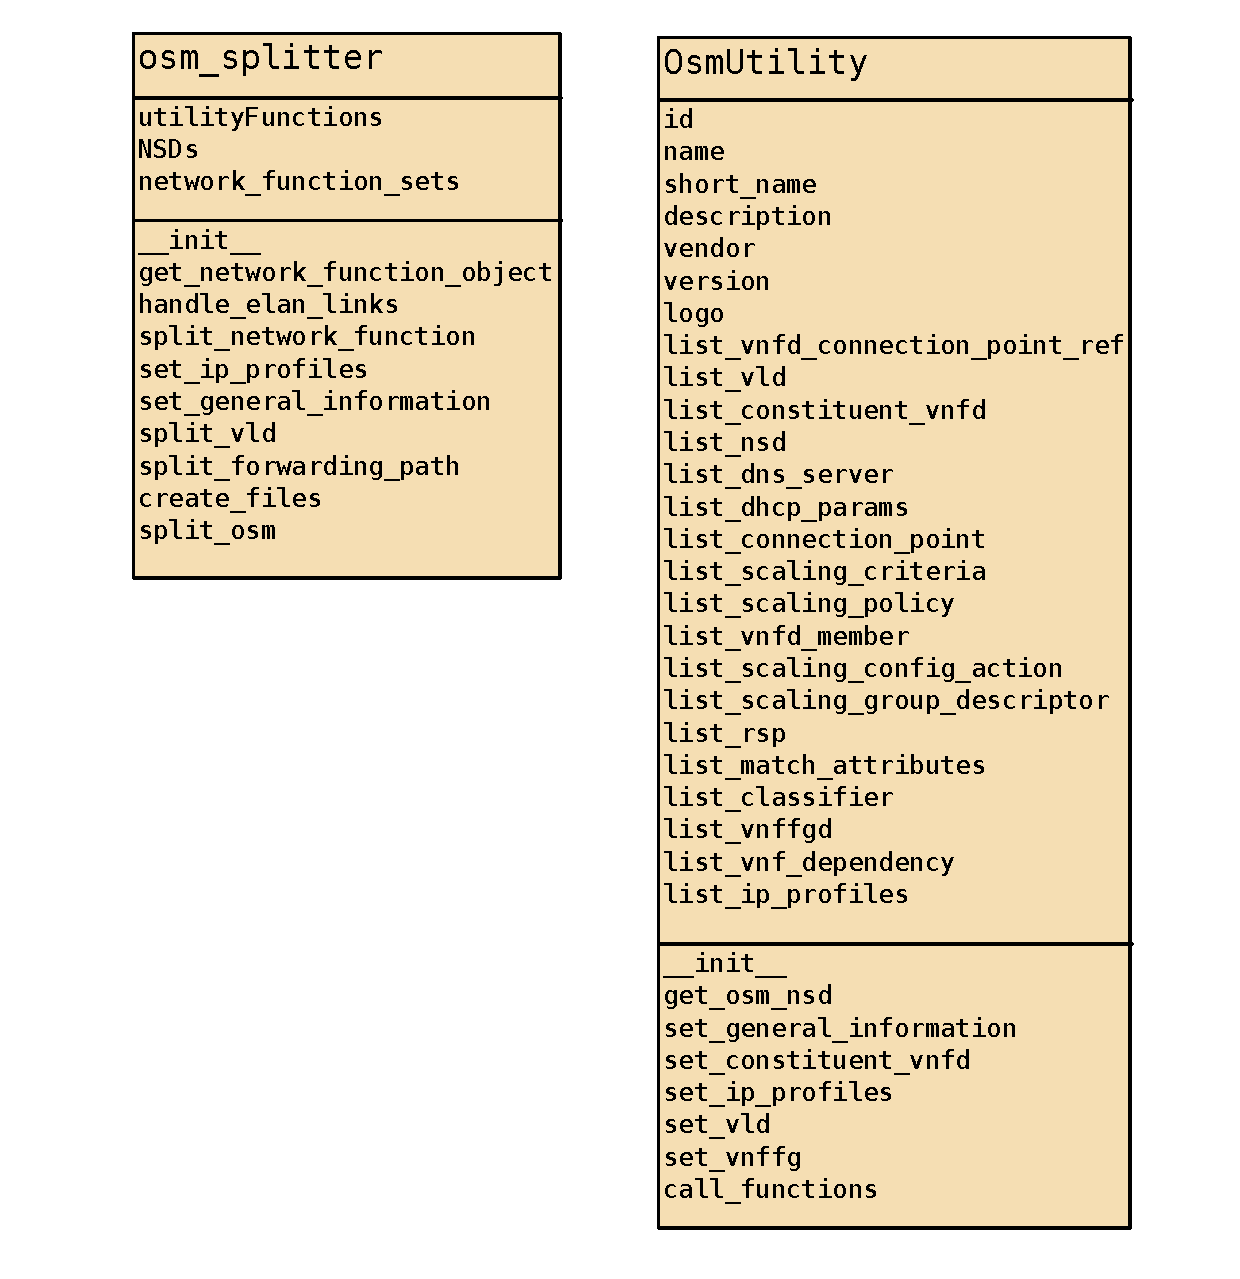
\includegraphics[width=1\linewidth]{../figures/OSM-Splitter}
	\caption{OSM Splitter Class diagram}
	\label{fig:osmsplitterclassdiagram}
\end{figure}

\begin{figure}
	\centering
	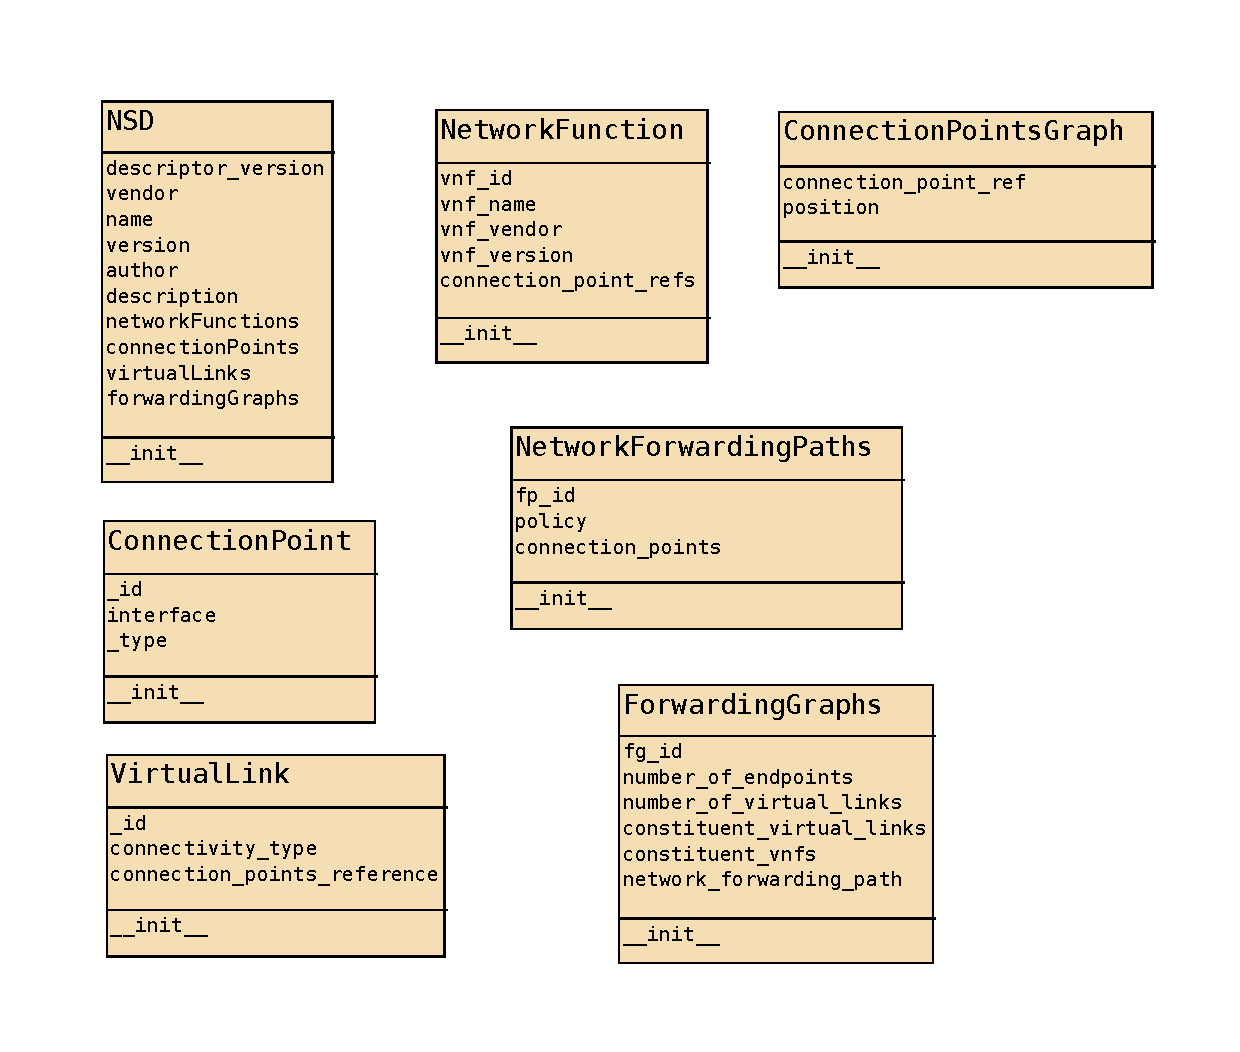
\includegraphics[width=1\linewidth]{../figures/pishahang-schema}
	\caption{Pishahang Schema Class Diagram}
	\label{fig:pishahangschemaclassdiagram}
\end{figure}

\begin{figure}
	\centering
	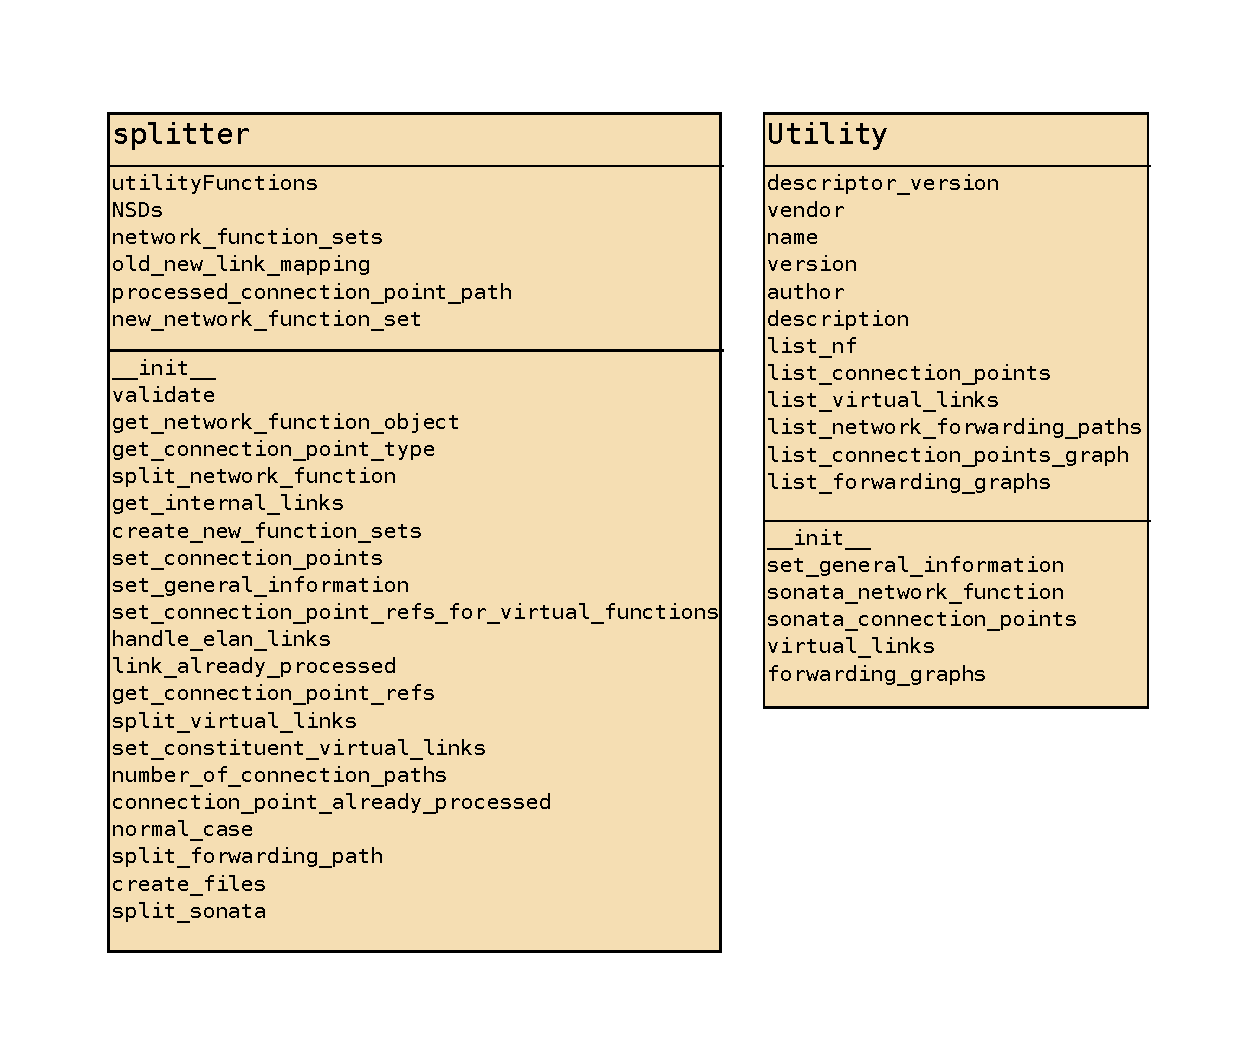
\includegraphics[width=1\linewidth]{../figures/Pishahang-Splitter}
	\caption{Pishahang Splitter Class diagram}
	\label{fig:pishahangsplitterclassdiagram}
\end{figure}

\begin{figure}
	\centering
	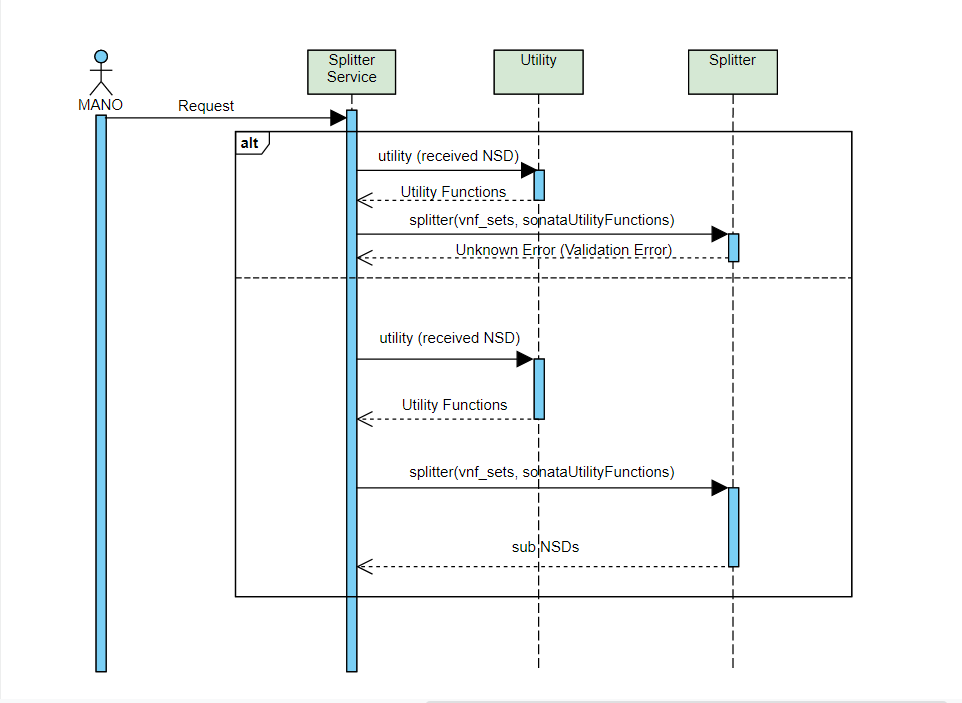
\includegraphics[width=1\linewidth]{../figures/splitter_sequence_diagram}
	\caption{Splitter Sequence diagram}
	\label{fig:splittersequencediagram}
\end{figure}



\subsection{Usage}

SDS is implemented as a micro-service which can be used independently from Translator or Wrapper by making a post call to the SDS. Following code snippet describes how to call SDS using POST call.

\begin{lstlisting}[caption=POST call to SDS, label=lis:postSDS]

splitter_url=http://$HOST:8003/Main_splitter/split

# Body: descriptor contains NSD, vnfid_set contains set of VNF ids
nsd = { 'descriptor' : descriptor, 'sets': vnfid_set}

LOG.info("Calling Scramble Splitter..." )
response  = requests.post(splitter_url,
data=json.dumps(nsd_to_split))

print(response)

\end{lstlisting}

Following are some of the important functions which helps SDS in splitting the NSD with respective code snippet.

\subsubsection{Python Base classes for NSD Schema} Following code snippet shows how NSD schema is mapped to various Python classes.

\begin{lstlisting}[caption=Python Base classes, label=lis:schemaclasses]

class NetworkFunction:  # class representing a network function and its properties
    vnf_id = ""
    vnf_name = ""
    vnf_vendor = ""
    vnf_version = ""
    connection_point_refs = []

    def __init__(self, vnf_id, vnf_vendor, vnf_name, vnf_version, connection_point_refs):
        self.vnf_id = vnf_id
        self.vnf_vendor = vnf_vendor
        self.vnf_name = vnf_name
        self.vnf_version = vnf_version
        self.connection_point_refs = connection_point_refs


class ConnectionPoint:  # class representing a connection point and its properties
    _id = ""
    interface = ""
    _type = ""

    def __init__(self, _id, interface, _type):
        self._id = _id
        self.interface = interface
        self._type = _type


class VirtualLink:  # class representing a virtual link and its properties
    _id = ""
    # connectivity type can be 'E-LAN' representing many to many connectivity or
    # 'E-Line' representing one to one
    connectivity_type = ""
    connection_points_reference = []

    def __init__(self, _id, connectivity_type, connection_points_reference):
        self._id = _id
        self.connectivity_type = connectivity_type
        self.connection_points_reference = connection_points_reference

\end{lstlisting}

\subsubsection{Splitting} "split sonata" calls the splitting function one by one to split the list of objects created out of NSD. Following code snippet shows the sequence of function calls.

\begin{lstlisting}[caption=Sequence of function calls, label=lis:functioncalls]

def split_sonata(self):
if self.validate() is not False:
self.create_new_function_sets()
self.set_connection_point_refs_for_virtual_functions()
self.split_network_function()
self.set_connection_points()
self.split_virtual_links()
self.split_forwarding_path()
self.set_general_information()
return self.create_files()
else:
print("Validation Failed!!")

\end{lstlisting}

\subsubsection{Validate} Validate method validates the request coming from the MANOs. For example, if MANO is requesting a NSD to be split into three parts but the original NSD contains just two VNFs then the SDS will throw validation error.

\begin{lstlisting}[caption=Splitting Request Validation, label=lis:validation]

def validate(self):
size = 0
list_network_function = []
for network_function_set in self.network_function_sets:
size = size + len(network_function_set)
for network_function in network_function_set:
list_network_function.append(network_function)

if size != len(self.utilityFunctions.list_nf):
return False
if len(list_network_function) != len(set(list_network_function)):
return False

\end{lstlisting}

\subsubsection{Split Network Functions}
This function updates the sub NSDs with set of network functions and there properties provided in the request.

\begin{lstlisting}[caption=Network Function Splitting, label=lis:NFSplitting]

def split_network_function(self):

for network_function_set in self.network_function_sets:

sub_nsd = SonataSchema.NSD("", "", "", "", "", "", [], [], [], [])

network_function_list = []

for network_function in network_function_set:

network_function_list.append(self.get_network_function_object(network_function))

sub_nsd.networkFunctions = network_function_list

self.NSDs.append(sub_nsd)

\end{lstlisting}

\subsubsection{Split Forwarding Graph} \label{fgsplitting}
The current implementation of splitter can successfully split a NSD with three or less VNFs.To maintain the topology of the main NSD, the graph has to consider the virtual links between VNFs present in the main NSD. The main challenge in splitting a forwarding graph is to maintain the topology. In case of four or more VNFs, the possible scenarios for splitting increases which increases the complexity of splitter. It can be achieved by maintaining a mapping of original one to one virtual links while processing the virtual links and then creating new virtual link set based on the request from MANO. Example, consider three VNFs, A, B and C. Packet is supposed to flow from A to B to C. After splitting, the sequence of packet flow should not be altered. If there is a request from MANO to split the NSD into two parts with [A, C] and [B], then to insure the topology is not changed, the NSD has to be splitted into three NSDs instead of two. In reference to the above example and following code snippet, normal scenario refers to when the request from MANO is to split it in such a way which does not result in creation of new virtual links which are not there in the original NSD. 

\begin{lstlisting}[caption=Forwarding Graph Splitting, label=lis:FGSplitting]

"""
    Method splits the forwarding path.
    """
    def split_forwarding_path(self):
        for i in range(len(self.NSDs)):
            nsd_fg = self.NSDs[i]
            del self.processed_connection_point_path[:]
            for fg in self.utilityFunctions.list_forwarding_graphs:
                
                fg_inner = SonataSchema.ForwardingGraphs(fg.fg_id, fg.number_of_endpoints,
                                               len(self.set_constituent_virtual_links(nsd_fg, fg)), self.network_function_sets[i],
                                               self.set_constituent_virtual_links(nsd_fg, fg), [])
                for path in fg.network_forwarding_path:
                    if self.number_of_connection_paths(self.set_constituent_virtual_links(nsd_fg, fg)) > 1:
                        for j in range(self.number_of_connection_paths(self.set_constituent_virtual_links(nsd_fg, fg))):
                            path_inner = SonataSchema.NetworkForwardingPaths(path.fp_id + "_" + str(j), path.policy, [])
                            x = 0
                            for cp in path.connection_points:
                                if self.connection_point_already_processed(cp.connection_point_ref) is False:
                                    found = 0
                                    if cp.connection_point_ref in self.get_connection_point_refs(nsd_fg.networkFunctions):
                                        x = x + 1
                                        point = SonataSchema.ConnectionPointsGraph(cp.connection_point_ref, x)
                                        path_inner.connection_points.append(point)
                                        found = 1
                                        self.processed_connection_point_path.append([cp.connection_point_ref, 1])
                                    else:
                                        for connection_point in nsd_fg.connectionPoints:
                                            if cp.connection_point_ref == connection_point._id:
                                                x = x + 1
                                                point = SonataSchema.ConnectionPointsGraph(cp.connection_point_ref, x)
                                                path_inner.connection_points.append(point)
                                                found = 1
                                                self.processed_connection_point_path.append([cp.connection_point_ref, 1])
                                    if found == 0:
                                        string = cp.connection_point_ref.split(":")
                                        if string[1] == "input":
                                            x = x + 1
                                            point = SonataSchema.ConnectionPointsGraph("output", x)
                                            path_inner.connection_points.append(point)
                                            self.processed_connection_point_path.append([cp.connection_point_ref, 1])
                                            break
                                        if string[1] == "output":
                                            x = 1
                                            point = SonataSchema.ConnectionPointsGraph("input", x)
                                            path_inner.connection_points.append(point)
                                            self.processed_connection_point_path.append([cp.connection_point_ref, 1])
                            fg_inner.network_forwarding_path.append(path_inner)
                    else:
                        fg_inner.network_forwarding_path.append(self.normal_case(path, nsd_fg))
                nsd_fg.forwardingGraphs.append(fg_inner)
            self.NSDs[i] = nsd_fg

\end{lstlisting}

\subsection{Challenges}
The NSD schema of Pishahang and OSM contains a lot of elements. However the challenge we faced was choosing which elements to include for splitting. We tackled it by including mandatory elements and a few optional elements mentioned in appendix \ref{psplitter} and \ref{osplitter} from the schema which were present in the input NSD.
\subsection{Future work}
SDS can currently split NSD of Pishahang and OSM. SDS is built in such a way that it can be implemented for new MANO frameworks as well. To implement SDS for a new MANO framework one can refer the implementation of either Pishahang or OSM. First step would be to create basic python classes from the NSD schema of the MANO framework then writing the utility functions to pull the information from the NSD file and store it in the objects of the basic python classes. Lastly writing splitting functions to actually split the list of objects in two or more parts.

Also, the current implementation considers all mandatory elements and a few optional elements from a NSD schema for splitting which can be extended to include other fields (Provided they are present in the input NSD for splitting).

Current implementation of SDS can split a forwarding graph of a NSD (Pishahang) with just three VNFs. Splitting of a forwarding graph is implemented by keeping future implementation for more than three VNFs in mind. (\ref{fgsplitting})
